\documentclass[12pt,a4paper]{article}

%% ─── PACKAGES ────────────────────────────────────────────────────────────────
\usepackage[T1]{fontenc}
\usepackage[utf8]{inputenc}
%\usepackage{microtype}

%% Math
\usepackage{amsmath,amssymb,amsthm,mathtools}
\usepackage{bm}           % bold math
% bbm not available — use \mathbf{1} for indicator

%% Layout & design
\usepackage[left=2.2cm,right=2.2cm,top=2.5cm,bottom=2.5cm]{geometry}
\usepackage{xcolor}
\usepackage{graphicx}
\usepackage{float}
\usepackage{caption}
\usepackage{subcaption}
\usepackage{booktabs}
\usepackage{array}
\usepackage{multirow}
\usepackage{longtable}
\usepackage{colortbl}
\usepackage{enumitem}
\usepackage{parskip}
\usepackage{setspace}
\usepackage{titlesec}
\usepackage{fancyhdr}
\usepackage{hyperref}
\usepackage{tcolorbox}
\usepackage{mdframed}
\usepackage{algorithm2e}
\usepackage{listings}
\usepackage{tikz}
\usepackage{pgfplots}
\pgfplotsset{compat=1.18}
\usetikzlibrary{arrows.meta,positioning,shapes,calc,decorations.pathreplacing}

%% ─── COLORS ──────────────────────────────────────────────────────────────────
\definecolor{navyblue}{HTML}{1a2340}
\definecolor{royalblue}{HTML}{2563eb}
\definecolor{lightblue}{HTML}{dbeafe}
\definecolor{midblue}{HTML}{60a5fa}
\definecolor{darkgray}{HTML}{374151}
\definecolor{lightgray}{HTML}{f3f4f6}
\definecolor{bordercolor}{HTML}{e5e7eb}
\definecolor{codebackground}{HTML}{f0f4ff}
\definecolor{codeborder}{HTML}{bfdbfe}
\definecolor{theorembg}{HTML}{fefce8}
\definecolor{theoremborder}{HTML}{ca8a04}
\definecolor{defbg}{HTML}{f0fdf4}
\definecolor{defborder}{HTML}{16a34a}
\definecolor{propbg}{HTML}{fdf4ff}
\definecolor{propborder}{HTML}{9333ea}
\definecolor{remarkbg}{HTML}{fff7ed}
\definecolor{remarkborder}{HTML}{ea580c}

%% ─── HYPERREF ────────────────────────────────────────────────────────────────
\hypersetup{
  colorlinks=true,
  linkcolor=royalblue,
  citecolor=royalblue,
  urlcolor=royalblue,
  pdftitle={Mini Framework ML From Scratch},
  pdfauthor={AHNANI Ali},
  pdfsubject={Mini Framework Machine Learning From Scratch}
}

%% ─── SECTION STYLING ─────────────────────────────────────────────────────────
\titleformat{\section}
  {\Large\bfseries\color{navyblue}}
  {\thesection.}{0.8em}{}
  [\vspace{-2pt}\color{royalblue}\rule{\linewidth}{1.5pt}]

\titleformat{\subsection}
  {\large\bfseries\color{navyblue}}
  {\thesubsection.}{0.6em}{}

\titleformat{\subsubsection}
  {\normalsize\bfseries\color{royalblue}}
  {\thesubsubsection.}{0.5em}{}

\titlespacing*{\section}{0pt}{18pt}{8pt}
\titlespacing*{\subsection}{0pt}{12pt}{5pt}
\titlespacing*{\subsubsection}{0pt}{8pt}{3pt}

%% ─── HEADER / FOOTER ─────────────────────────────────────────────────────────
\pagestyle{fancy}
\fancyhf{}
\fancyhead[L]{\small\color{navyblue}\textbf{Mini Framework ML — From Scratch}}
\fancyhead[R]{\small\color{darkgray}AHNANI Ali}
\fancyfoot[C]{\small\color{darkgray}\thepage}
\fancyfoot[L]{\small\color{darkgray}Python + NumPy uniquement}
\renewcommand{\headrulewidth}{1pt}
\renewcommand{\headrule}{\hbox to\headwidth{\color{royalblue}\leaders\hrule height \headrulewidth\hfill}}

%% ─── TCOLORBOX ENVIRONMENTS ──────────────────────────────────────────────────
\tcbuselibrary{skins,breakable,theorems}

\newtcolorbox{theorembox}[1][]{
  enhanced, breakable,
  colback=theorembg, colframe=theoremborder,
  fonttitle=\bfseries\color{white},
  title=#1,
  attach boxed title to top left={yshift=-2mm,xshift=4mm},
  boxed title style={colback=theoremborder, rounded corners},
  rounded corners, arc=4pt,
  left=6pt, right=6pt, top=8pt, bottom=6pt
}

\newtcolorbox{definitionbox}[1][]{
  enhanced, breakable,
  colback=defbg, colframe=defborder,
  fonttitle=\bfseries\color{white},
  title=#1,
  attach boxed title to top left={yshift=-2mm,xshift=4mm},
  boxed title style={colback=defborder, rounded corners},
  rounded corners, arc=4pt,
  left=6pt, right=6pt, top=8pt, bottom=6pt
}

\newtcolorbox{propbox}[1][]{
  enhanced, breakable,
  colback=propbg, colframe=propborder,
  fonttitle=\bfseries\color{white},
  title=#1,
  attach boxed title to top left={yshift=-2mm,xshift=4mm},
  boxed title style={colback=propborder, rounded corners},
  rounded corners, arc=4pt,
  left=6pt, right=6pt, top=8pt, bottom=6pt
}

\newtcolorbox{remarkbox}[1][Remarque]{
  enhanced, breakable,
  colback=remarkbg, colframe=remarkborder,
  fonttitle=\bfseries\color{white},
  title=#1,
  attach boxed title to top left={yshift=-2mm,xshift=4mm},
  boxed title style={colback=remarkborder, rounded corners},
  rounded corners, arc=4pt,
  left=6pt, right=6pt, top=8pt, bottom=6pt
}

\newtcolorbox{codebox}[1][]{
  enhanced, breakable,
  colback=codebackground, colframe=codeborder,
  fonttitle=\bfseries\color{navyblue}\small,
  title=#1,
  rounded corners, arc=4pt,
  left=8pt, right=8pt, top=6pt, bottom=6pt,
  fontupper=\ttfamily\small\color{navyblue}
}

\newtcolorbox{infobox}{
  enhanced,
  colback=lightblue, colframe=royalblue,
  rounded corners, arc=4pt,
  left=8pt, right=8pt, top=6pt, bottom=6pt,
  fontupper=\small\color{navyblue}
}

%% ─── LISTINGS (code) ─────────────────────────────────────────────────────────
\lstset{
  language=Python,
  backgroundcolor=\color{codebackground},
  basicstyle=\ttfamily\footnotesize\color{navyblue},
  keywordstyle=\bfseries\color{royalblue},
  commentstyle=\itshape\color{darkgray},
  stringstyle=\color{defborder},
  numbers=left,
  numberstyle=\tiny\color{darkgray},
  numbersep=8pt,
  frame=single,
  framesep=4pt,
  rulecolor=\color{codeborder},
  breaklines=true,
  showstringspaces=false,
  tabsize=4,
  captionpos=b,
  belowskip=6pt,
  aboveskip=6pt
}

%% ─── MATH COMMANDS ───────────────────────────────────────────────────────────
\newcommand{\R}{\mathbb{R}}
\newcommand{\E}{\mathbb{E}}
\newcommand{\norm}[1]{\left\|#1\right\|}
\newcommand{\abs}[1]{\left|#1\right|}
\newcommand{\inner}[2]{\langle #1,\, #2 \rangle}
\newcommand{\grad}{\nabla}
\newcommand{\Hess}{\nabla^2}
\newcommand{\T}{\mathsf{T}}
\newcommand{\eye}{\mathbf{I}}
\newcommand{\zeros}{\mathbf{0}}
\newcommand{\ones}{\mathbf{1}}
\newcommand{\bx}{\mathbf{x}}
\newcommand{\by}{\mathbf{y}}
\newcommand{\bw}{\mathbf{w}}
\newcommand{\bW}{\mathbf{W}}
\newcommand{\bb}{\mathbf{b}}
\newcommand{\bz}{\mathbf{z}}
\newcommand{\ba}{\mathbf{a}}
\newcommand{\bh}{\mathbf{h}}
\newcommand{\bg}{\mathbf{g}}
\newcommand{\bd}{\mathbf{d}}
\newcommand{\bG}{\mathbf{G}}
\newcommand{\bK}{\mathbf{K}}
\newcommand{\balpha}{\bm{\alpha}}
\newcommand{\blambda}{\bm{\lambda}}
\newcommand{\btheta}{\bm{\theta}}
\newcommand{\sigmoid}{\sigma}
\newcommand{\softmax}{\mathrm{softmax}}
\newcommand{\relu}{\mathrm{ReLU}}
\newcommand{\gelu}{\mathrm{GELU}}
\newcommand{\BCE}{\mathcal{L}_{\mathrm{BCE}}}
\newcommand{\CE}{\mathcal{L}_{\mathrm{CE}}}
\newcommand{\KL}{\mathrm{KL}}
\newcommand{\tr}{\mathrm{tr}}
\newcommand{\diag}{\mathrm{diag}}
\newcommand{\Od}{\mathcal{O}}
\newcommand{\cH}{\mathcal{H}}
\newcommand{\cF}{\mathcal{F}}
\newcommand{\cL}{\mathcal{L}}
\newcommand{\eps}{\varepsilon}
\newcommand{\indic}[1]{\mathbf{1}\!\left[#1\right]}

%% ─── THEOREM ENVIRONMENTS ────────────────────────────────────────────────────
\theoremstyle{plain}
\newtheorem{theorem}{Théorème}[section]
\newtheorem{proposition}{Proposition}[section]
\newtheorem{corollary}{Corollaire}[section]
\newtheorem{lemma}{Lemme}[section]

\theoremstyle{definition}
\newtheorem{definition}{Définition}[section]
\newtheorem{example}{Exemple}[section]

\theoremstyle{remark}
\newtheorem{remark}{Remarque}[section]

%% ─── CAPTION STYLE ───────────────────────────────────────────────────────────
\captionsetup{
  font=small, labelfont={bf,color=navyblue},
  textfont={it,color=darkgray},
  labelsep=period
}

%% ─── DOCUMENT ────────────────────────────────────────────────────────────────
\begin{document}

%% ══════════════════════════════════════════════════════════════════════════════
%%  PAGE DE GARDE
%% ══════════════════════════════════════════════════════════════════════════════
\begin{titlepage}

\begin{tikzpicture}[remember picture, overlay]
  %% Background
  \fill[navyblue] (current page.south west) rectangle (current page.north east);
  %% Top accent
  \fill[royalblue] (current page.north west) rectangle
    ([yshift=-3.5cm] current page.north east);
  \fill[midblue] ([yshift=-3.5cm] current page.north west)
    rectangle ([yshift=-3.7cm] current page.north east);
  %% Bottom accent
  \fill[royalblue] (current page.south west) rectangle
    ([yshift=2.2cm] current page.south east);
  %% Side stripe
  \fill[royalblue!60] ([xshift=0cm] current page.south west)
    rectangle ([xshift=0.5cm] current page.north west);
  %% Decorative circle
  \fill[royalblue!30,opacity=0.3]
    ([xshift=12cm,yshift=-10cm] current page.north west) circle (6cm);
  \fill[royalblue!20,opacity=0.2]
    ([xshift=3cm,yshift=-16cm] current page.north west) circle (4cm);
\end{tikzpicture}

\vspace*{1.5cm}

\begin{center}
  {\fontsize{11}{13}\selectfont\color{midblue}\textbf{MINI FRAMEWORK MACHINE LEARNING}}\\[0.4cm]
  {\fontsize{10}{12}\selectfont\color{lightblue!70}\textit{Implémentation complète from scratch — Python + NumPy}}

  \vspace{1.2cm}
  \color{bordercolor}\rule{12cm}{0.5pt}
  \vspace{0.6cm}

  {\fontsize{36}{42}\selectfont\bfseries\color{white}Mini Framework}\\[0.3cm]
  {\fontsize{36}{42}\selectfont\bfseries\color{midblue}Machine Learning}\\[0.2cm]
  {\fontsize{20}{24}\selectfont\color{lightblue}\textit{From Scratch}}

  \vspace{0.6cm}
  \color{bordercolor}\rule{12cm}{0.5pt}
  \vspace{0.8cm}

  {\fontsize{12}{14}\selectfont\color{lightblue}
    Autodiff \(\cdot\) Optimiseurs \(\cdot\) MLP Profond \(\cdot\) Kernel Ridge \(\cdot\) MNIST}

  \vspace{1.8cm}

  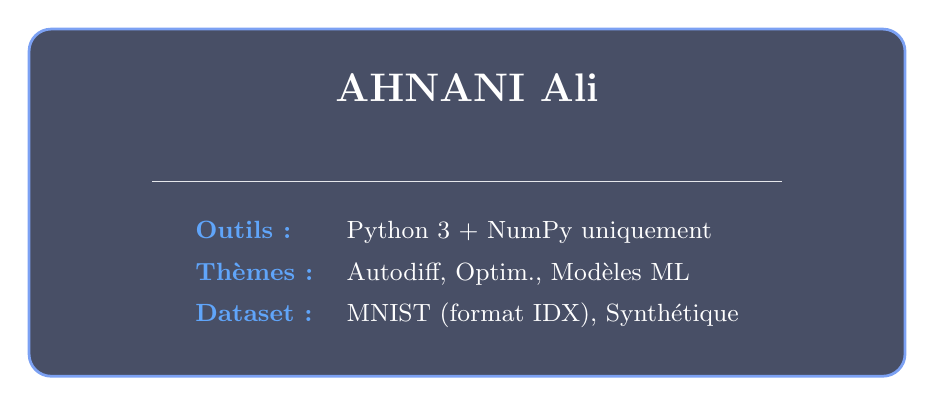
\begin{tikzpicture}
    \node[draw=royalblue!60, fill=navyblue!80, rounded corners=8pt,
          inner sep=16pt, line width=1pt] {
      \begin{minipage}{10cm}
        \centering
        {\Large\bfseries\color{white} AHNANI Ali}\\[0.6cm]
        \color{bordercolor}\rule{8cm}{0.3pt}\\[0.4cm]
        \begin{tabular}{ll}
          \color{midblue}\small\textbf{Outils :}    & \color{white}\small Python 3 + NumPy uniquement \\[3pt]
          \color{midblue}\small\textbf{Thèmes :}    & \color{white}\small Autodiff, Optim., Modèles ML \\[3pt]
          \color{midblue}\small\textbf{Dataset :}   & \color{white}\small MNIST (format IDX), Synthétique \\
        \end{tabular}
      \end{minipage}
    };
  \end{tikzpicture}

  \vspace{2cm}

  \begin{tabular}{p{1.8cm}p{10cm}}
    \cellcolor{royalblue}\centering\color{white}\small\textbf{P.1} &
      \cellcolor{navyblue!80}\small\color{lightblue} Moteur Autodiff — Graphe computationnel dynamique + backward\\[3pt]
    \cellcolor{royalblue!70}\centering\color{white}\small\textbf{P.2} &
      \cellcolor{navyblue!80}\small\color{lightblue} Optimiseurs — SGD, Momentum, RMSProp, Adam (théorie + convergence)\\[3pt]
    \cellcolor{royalblue}\centering\color{white}\small\textbf{P.3} &
      \cellcolor{navyblue!80}\small\color{lightblue} Modèles — Logistique, MLP Profond, Kernel Ridge Regression\\[3pt]
    \cellcolor{royalblue!70}\centering\color{white}\small\textbf{P.4} &
      \cellcolor{navyblue!80}\small\color{lightblue} Dataset — MNIST manuel format IDX, jeux de données synthétiques\\[3pt]
    \cellcolor{royalblue}\centering\color{white}\small\textbf{P.5} &
      \cellcolor{navyblue!80}\small\color{lightblue} Expériences — Optimiseurs, LR, Régularisation, Comparaison modèles\\[3pt]
    \cellcolor{royalblue!70}\centering\color{white}\small\textbf{P.6} &
      \cellcolor{navyblue!80}\small\color{lightblue} Complexité — Analyse algorithmique empirique et théorique\\[3pt]
    \cellcolor{royalblue}\centering\color{white}\small\textbf{+} &
      \cellcolor{navyblue!80}\small\color{lightblue} Fonctionnalités Avancées — Scheduler, Early Stopping, Gradient Clipping, NTK\\
  \end{tabular}

  \vfill
  {\small\color{lightblue!60}\textit{AHNANI Ali}}
\end{center}
\end{titlepage}

\newpage
\setcounter{page}{1}

%% ── TABLE DES MATIÈRES ────────────────────────────────────────────────────────
{
\hypersetup{linkcolor=navyblue}
\tableofcontents
}
\newpage

%% ══════════════════════════════════════════════════════════════════════════════
%%  INTRODUCTION
%% ══════════════════════════════════════════════════════════════════════════════
\section{Introduction}

Ce rapport présente la conception et l'implémentation d'un \textbf{mini-framework de Machine Learning complet} en Python pur, en utilisant uniquement NumPy pour les opérations numériques. L'objectif est triple : comprendre en profondeur les mécanismes fondamentaux du ML moderne, en fournir une analyse mathématique rigoureuse, et valider empiriquement les propriétés théoriques.

\begin{infobox}
\textbf{Contrainte fondamentale :} aucune bibliothèque ML externe (PyTorch, TensorFlow, scikit-learn, JAX). Chaque brique algorithmique est construite \textit{from scratch} à partir des mathématiques.
\end{infobox}

Le pipeline couvre six composantes essentielles : un moteur de différentiation automatique (autodiff), quatre optimiseurs avec analyse de convergence, trois familles de modèles (régression paramétrique, réseaux profonds, méthodes à noyaux), un chargeur de données MNIST au format IDX, des expériences comparatives rigoureuses, et une analyse de complexité algorithmique empiriquement validée.

%% ══════════════════════════════════════════════════════════════════════════════
%%  PARTIE 1 — AUTODIFF
%% ══════════════════════════════════════════════════════════════════════════════
\section{Moteur de Différentiation Automatique}

\subsection{Fondements mathématiques}

\subsubsection{Graphe computationnel et règle de la chaîne}

Soit $f : \R^n \to \R$ une fonction composite $f = f_L \circ f_{L-1} \circ \cdots \circ f_1$. On représente le calcul par un \textbf{graphe orienté acyclique} (DAG) $G = (V, E)$ où chaque nœud $v \in V$ correspond à une variable intermédiaire $z_v$, et chaque arête $(u, v) \in E$ indique que $z_v$ dépend de $z_u$.

\begin{definitionbox}[Différentiation Automatique — Mode Reverse]
Soit $L = f(\bx)$ la loss scalaire. Pour tout nœud $v$, on définit le \textit{gradient accumulé} (ou sensibilité) :
\[
\bar{z}_v \;=\; \frac{\partial L}{\partial z_v}
\]
Le mode reverse calcule tous les $\bar{z}_v$ en un seul passage backward depuis le nœud de sortie, grâce à la règle de la chaîne généralisée :
\[
\bar{z}_v \;=\; \sum_{w \,:\, (v,w)\in E} \bar{z}_w \cdot \frac{\partial z_w}{\partial z_v}
\]
\end{definitionbox}

\subsubsection{Tri topologique et accumulation}

\begin{theorembox}[Correction du backward par tri topologique]
Soit $G = (V,E)$ le DAG computationnel. L'ordre de traitement backward est donné par l'ordre topologique \emph{renversé} de $G$, c'est-à-dire tout ordre tel que si $(u,v) \in E$ alors $v$ est traité avant $u$ en backward.

Sous cet ordre, chaque fois que le backward de $v$ est appelé, tous les $\bar{z}_w$ pour $w$ descendant de $v$ sont déjà calculés et accumulés. L'algorithme est donc \textbf{correct}.
\end{theorembox}

\textbf{Preuve.} Par induction sur l'ordre topologique. Pour le nœud de sortie $L$, on pose $\bar{L} = 1$. Pour tout nœud $v$ traité à l'étape $k$, tous ses descendants ont été traités aux étapes $< k$ (par définition du tri topologique renversé). Donc $\bar{z}_v$ est complètement accumulé avant qu'on l'utilise. \hfill$\square$

\subsubsection{Algorithme complet}

\begin{algorithm}[H]
\SetAlgoLined
\KwIn{Nœud de sortie $L$ (scalaire)}
\KwOut{Gradients $\bar{z}_v = \partial L / \partial z_v$ pour tout $v \in V$}
\BlankLine
\tcp{Phase 1 : Construction de l'ordre topologique}
$\text{topo} \leftarrow [\;]$\;
$\text{visited} \leftarrow \emptyset$\;
\SetKwFunction{FBuildTopo}{BuildTopo}
\SetKwProg{Fn}{Fonction}{:}{}
\Fn{\FBuildTopo{$v$}}{
  \If{$v \notin \text{visited}$}{
    $\text{visited} \leftarrow \text{visited} \cup \{v\}$\;
    \For{$u \in \text{parents}(v)$}{
      \FBuildTopo{$u$}\;
    }
    $\text{topo}.\text{append}(v)$\;
  }
}
\FBuildTopo{$L$}\;
\BlankLine
\tcp{Phase 2 : Propagation backward}
$\bar{z}_L \leftarrow 1$ \tcp*{$\partial L / \partial L = 1$}
\For{$v \in \text{reversed}(\text{topo})$}{
  Appeler $v.\text{\_backward}()$ \tcp*{accumule $\bar{z}_u \mathrel{+}= \bar{z}_v \cdot \partial z_v/\partial z_u$ pour tout parent $u$}
}
\caption{Reverse-Mode Autodiff (Backpropagation généralisée)}
\end{algorithm}

\subsubsection{Gradients des opérations fondamentales}

Voici les formules analytiques des gradients locaux pour les principales opérations :

\begin{center}
\renewcommand{\arraystretch}{1.5}
\begin{tabular}{@{}lllc@{}}
\toprule
\textbf{Opération} & \textbf{Forward} $z_v$ & \textbf{Gradient local} $\partial z_v / \partial z_u$ & \textbf{Coût backward} \\
\midrule
Addition & $\ba + \bb$ & $\partial/\partial\ba = \bm{1}$, $\partial/\partial\bb = \bm{1}$ & $\Od(n)$ \\
Multiplication & $\ba \odot \bb$ & $\partial/\partial\ba = \bb$, $\partial/\partial\bb = \ba$ & $\Od(n)$ \\
Matmul & $\mathbf{A}\mathbf{B}$ & $\partial/\partial\mathbf{A} = \bG \mathbf{B}^\T$, $\partial/\partial\mathbf{B} = \mathbf{A}^\T \bG$ & $\Od(ndk)$ \\
Exponentielle & $e^{\bx}$ & $e^{\bx}$ & $\Od(n)$ \\
Logarithme & $\log \bx$ & $\bx^{-1}$ & $\Od(n)$ \\
ReLU & $\max(\zeros, \bx)$ & $\indic{}[\bx > 0]$ & $\Od(n)$ \\
GELU & $\bx \cdot \sigmoid(1.702\bx)$ & voir ci-dessous & $\Od(n)$ \\
Somme & $\sum_i x_i$ & $\ones^\T$ (broadcast) & $\Od(n)$ \\
Puissance & $\bx^k$ & $k \bx^{k-1}$ & $\Od(n)$ \\
\bottomrule
\end{tabular}
\end{center}

\textbf{Gradient de GELU.} En posant $\sigmoid(x) = (1 + e^{-x})^{-1}$ et $s = \sigmoid(1.702 x)$ :
\[
\gelu'(x) = s + x \cdot 1.702 \cdot s(1-s)
\]

\subsubsection{Gestion du broadcasting NumPy}

Lorsqu'une opération implique un broadcast (ex. ajouter un biais de forme $(1, d)$ à une activation de forme $(n, d)$), le gradient doit être \textbf{réduit (sommé)} sur les axes broadcastés pour retrouver la forme originale. Formellement, si $z = \ba + \bb$ avec $\ba \in \R^{n \times d}$ et $\bb \in \R^{1 \times d}$ :
\[
\bar{\bb} \mathrel{+}= \sum_{i=1}^{n} \bar{z}_{i,:}
\]

\subsubsection{Complexité}

\begin{propbox}[Complexité de l'autodiff]
Pour un graphe computationnel $G = (V, E)$ :
\begin{itemize}[leftmargin=1.5em]
  \item \textbf{Temps forward} : $\Od(|V| + |E|)$ — proportionnel à la taille du graphe.
  \item \textbf{Temps backward} : $\Od(|V| + |E|)$ — même ordre que le forward.
  \item \textbf{Mémoire} : $\Od(|V|)$ — on stocke toutes les activations intermédiaires pour le backward.
\end{itemize}
En pratique, pour un MLP de $L$ couches de largeur $d$ et batch $n$ : $|V| = \Od(L)$, et le coût dominant est $\Od(L n d^2)$ (matmul).
\end{propbox}

\begin{figure}[H]
  \centering
  \includegraphics[width=0.72\textwidth]{fig_graph_complexity.png}
  \caption{Croissance de la taille du graphe computationnel en fonction de la profondeur. La linéarité confirme $\Od(|\text{graph}|)$ en mémoire.}
  \label{fig:graph}
\end{figure}

\subsection{Implémentation de la classe \texttt{Tensor}}

\begin{lstlisting}[caption={Classe Tensor — structure et opération matmul avec backward}, label=lst:tensor]
class Tensor:
    def __init__(self, data, _children=(), _op=''):
        self.data = np.array(data, dtype=np.float64)
        self.grad = np.zeros_like(self.data)   # gradient accumule
        self._backward = lambda: None           # fonction backward locale
        self._prev = set(_children)             # parents dans le graphe

    def __matmul__(self, other):
        # Forward : C = A @ B
        out = Tensor(self.data @ other.data, (self, other), 'matmul')
        def _backward():
            # dL/dA = dL/dC @ B^T,   dL/dB = A^T @ dL/dC
            self.grad  += out.grad @ other.data.T
            other.grad += self.data.T @ out.grad
        out._backward = _backward
        return out

    def backward(self):
        topo = []; visited = set()
        def build_topo(v):
            if id(v) not in visited:
                visited.add(id(v))
                for child in v._prev: build_topo(child)
                topo.append(v)
        build_topo(self)
        self.grad = np.ones_like(self.data)  # dL/dL = 1
        for node in reversed(topo):
            node._backward()
\end{lstlisting}

\newpage
%% ══════════════════════════════════════════════════════════════════════════════
%%  PARTIE 2 — OPTIMISEURS
%% ══════════════════════════════════════════════════════════════════════════════
\section{Optimiseurs — Théorie et Implémentation}

\subsection{Gradient Descent Stochastique (SGD)}

\subsubsection{Formulation}

Soit $\cL(\btheta) = \E_{(\bx,y)\sim\mathcal{D}}[\ell(f_{\btheta}(\bx), y)]$ la loss attendue. Le SGD met à jour les paramètres selon :
\[
\btheta_{t+1} = \btheta_t - \eta \grad_{\btheta} \cL_{\mathcal{B}_t}(\btheta_t)
\]
où $\mathcal{B}_t$ est un mini-batch aléatoire de taille $B$ et $\eta > 0$ le taux d'apprentissage.

\subsubsection{Convergence}

\begin{theorembox}[Convergence SGD — Fonctions Convexes]
Supposons $\cL$ convexe, $G$-Lipschitz ($\norm{\grad\cL} \leq G$), et $\norm{\btheta_0 - \btheta^*} \leq D$. Avec $\eta_t = \eta / \sqrt{t}$, le SGD vérifie :
\[
\E\left[\cL\!\left(\frac{1}{T}\sum_{t=1}^T \btheta_t\right)\right] - \cL(\btheta^*) \;\leq\; \frac{DG}{\sqrt{T}}
\]
donc un taux de convergence $\Od(1/\sqrt{T})$ en général, et $\Od(1/T)$ si $\cL$ est fortement convexe ($\mu > 0$).
\end{theorembox}

\subsubsection{SGD avec Momentum (Polyak)}

L'ajout du momentum accélère la convergence dans les directions de gradient cohérentes :
\[
\mathbf{v}_{t+1} = \beta\, \mathbf{v}_t + \grad\cL(\btheta_t), \qquad \btheta_{t+1} = \btheta_t - \eta\, \mathbf{v}_{t+1}
\]
Pour des fonctions $\mu$-fortement convexes et $L$-lisses, le momentum réduit le taux de convergence de $\Od\!\big((L/\mu)^2\big)$ à $\Od\!\big(L/\mu\big)$ en nombre d'itérations.

\subsection{RMSProp}

Proposé par Tieleman \& Hinton (2012), RMSProp adapte le learning rate par paramètre via une moyenne mobile du carré des gradients :
\[
v_{t+1}^{(i)} = \rho\, v_t^{(i)} + (1-\rho)\, \big(\grad_i \cL(\btheta_t)\big)^2
\]
\[
\theta_{t+1}^{(i)} = \theta_t^{(i)} - \frac{\eta}{\sqrt{v_{t+1}^{(i)}} + \epsilon}\, \grad_i \cL(\btheta_t)
\]
La normalisation par $\sqrt{v_t}$ précondionne implicitement le gradient, ce qui est particulièrement efficace pour les paysages de loss à courbure hétérogène.

\subsection{Adam — Adaptive Moment Estimation}

\subsubsection{Algorithme}

Adam (Kingma \& Ba, 2014) combine le momentum du premier ordre et l'adaptation du second ordre :

\begin{align}
m_{t+1} &= \beta_1 m_t + (1-\beta_1)\, \bg_t \quad \text{(premier moment)}\\
v_{t+1} &= \beta_2 v_t + (1-\beta_2)\, \bg_t^2 \quad \text{(second moment)}\\
\hat{m}_{t+1} &= \frac{m_{t+1}}{1 - \beta_1^{t+1}}, \quad \hat{v}_{t+1} = \frac{v_{t+1}}{1 - \beta_2^{t+1}} \quad \text{(correction biais)}\\
\btheta_{t+1} &= \btheta_t - \eta \cdot \frac{\hat{m}_{t+1}}{\sqrt{\hat{v}_{t+1}} + \epsilon}
\end{align}

\subsubsection{Justification de la correction du biais}

Sans correction, $m_0 = \zeros$ implique un biais initial : $\E[m_1] = (1-\beta_1)\bg$, soit un sous-estimation par facteur $(1-\beta_1)$. La correction $\hat{m}_t = m_t/(1-\beta_1^t)$ compense cet effet de départ à froid.

\begin{propbox}[Invariance à l'échelle d'Adam]
Si on multiplie tous les gradients par une constante $c > 0$ (changement d'échelle de la loss), la mise à jour d'Adam est \textbf{inchangée} (car $\hat{m}$ et $\sqrt{\hat{v}}$ sont multipliés par $c$ et $\sqrt{c}$ respectivement, et le rapport $\hat{m}/\sqrt{\hat{v}}$ dépend de l'historique des directions).

Cette propriété rend Adam robuste aux changements d'échelle de la loss, contrairement au SGD.
\end{propbox}

\subsection{Tableau comparatif des optimiseurs}

\begin{center}
\renewcommand{\arraystretch}{1.4}
\begin{tabular}{@{}lllllc@{}}
\toprule
\textbf{Méthode} & \textbf{Mise à jour} & \textbf{Coût/step} & \textbf{Mémoire} & \textbf{Convergence} & \textbf{Adaptatif} \\
\midrule
SGD             & $\btheta - \eta\bg$                         & $\Od(p)$  & $\Od(p)$  & $\Od(1/\sqrt{T})$    & Non \\
Momentum        & $\btheta - \eta\mathbf{v}$                         & $\Od(p)$  & $\Od(2p)$ & $\Od(1/T)$ s.c.      & Non \\
RMSProp         & $\btheta - \eta\bg/\sqrt{v+\epsilon}$        & $\Od(p)$  & $\Od(2p)$ & Empirique            & Oui \\
Adam            & $\btheta - \eta\hat{m}/(\sqrt{\hat{v}}+\eps)$ & $\Od(p)$ & $\Od(3p)$ & Empirique            & Oui \\
\bottomrule
\end{tabular}
\end{center}

\begin{figure}[H]
  \centering
  \includegraphics[width=\textwidth]{fig_optimizers.png}
  \caption{Benchmark sur la fonction de Rosenbrock $f(x,y)=(1-x)^2+100(y-x^2)^2$ (minimum en $(1,1)$, vallée très courbée). Adam converge le plus rapidement. SGD pur reste bloqué dans la vallée.}
  \label{fig:optimizers}
\end{figure}

\newpage
%% ══════════════════════════════════════════════════════════════════════════════
%%  PARTIE 3a — LOGISTIC
%% ══════════════════════════════════════════════════════════════════════════════
\section{Modèles ML From Scratch}

\subsection{Régression Logistique}

\subsubsection{Modèle probabiliste}

La régression logistique modélise la probabilité conditionnelle $P(y=1|\bx; \bw, b)$ par une sigmoïde :
\[
\hat{p} = \sigmoid(\bw^\T \bx + b) = \frac{1}{1 + e^{-(\bw^\T\bx + b)}}
\]
où $\sigmoid : \R \to (0,1)$ est la fonction sigmoïde. Ce choix correspond à un modèle de la famille exponentielle (distribution de Bernoulli avec lien logit).

\subsubsection{Fonction de perte — Binary Cross-Entropy}

La BCE est dérivée du principe du \textbf{maximum de vraisemblance} :
\[
\BCE(\bw) = -\frac{1}{n}\sum_{i=1}^n \Big[ y_i \log \hat{p}_i + (1-y_i)\log(1-\hat{p}_i) \Big]
\]
Equivalence avec la divergence KL : $\BCE(\bw) = \KL\!\big(P_{\text{data}} \,\|\, P_{\bw}\big) + H(P_{\text{data}})$, donc minimiser la BCE revient à minimiser la divergence KL entre la distribution empirique et le modèle.

\subsubsection{Convexité et convergence garantie}

\begin{theorembox}[Convexité de la BCE]
La loss $\BCE(\bw)$ est une fonction \textbf{convexe} de $\bw$. Sa Hessienne est :
\[
\Hess \BCE(\bw) = \frac{1}{n}\sum_{i=1}^n \hat{p}_i(1-\hat{p}_i)\, \bx_i \bx_i^\T = \frac{1}{n} \mathbf{X}^\T \mathbf{S} \mathbf{X}
\]
où $\mathbf{S} = \diag\!\big(\hat{p}_i(1-\hat{p}_i)\big) \succeq 0$. Donc $\Hess \BCE \succeq 0$, ce qui établit la convexité.
\end{theorembox}

\begin{corollary}
Le gradient descent converge vers le minimum global de $\BCE$, qui est unique si $\mathbf{X}$ est de plein rang colonne. Le taux de convergence est $\Od(1/T)$ pour GD classique.
\end{corollary}

\textbf{Gradient analytique :}
\[
\grad_{\bw} \BCE = \frac{1}{n} \mathbf{X}^\T (\hat{\mathbf{p}} - \mathbf{y}) = \frac{1}{n}\sum_{i=1}^n (\hat{p}_i - y_i)\, \bx_i
\]
Ce gradient est calculé automatiquement par notre moteur autodiff.

\begin{figure}[H]
  \centering
  \includegraphics[width=\textwidth]{fig_logistic.png}
  \caption{Régression Logistique : convergence BCE (gauche), accuracy test (centre), frontière de décision (droite). La convexité garantit la convergence vers l'optimum global.}
  \label{fig:logistic}
\end{figure}

\subsection{MLP Profond (Deep Neural Network)}

\subsubsection{Architecture et notation}

Un MLP à $L$ couches cachées définit une fonction $f_{\btheta} : \R^{d_0} \to \R^{d_L}$ par :
\begin{align}
\bz^{(0)} &= \bx \in \R^{d_0} \\
\bz^{(\ell)} &= \phi\!\big(\bW^{(\ell)} \bz^{(\ell-1)} + \bb^{(\ell)}\big), \quad \ell = 1, \ldots, L-1 \\
\bz^{(L)} &= \bW^{(L)} \bz^{(L-1)} + \bb^{(L)} \in \R^{d_L} \quad \text{(logits)}
\end{align}
où $\phi$ est une fonction d'activation non-linéaire, $\bW^{(\ell)} \in \R^{d_\ell \times d_{\ell-1}}$ et $\bb^{(\ell)} \in \R^{d_\ell}$.

\subsubsection{Fonctions d'activation}

\textbf{ReLU (Nair \& Hinton, 2010) :}
\[
\relu(x) = \max(0, x), \qquad \relu'(x) = \indic{}[x > 0]
\]
Avantage : gradient non-saturant pour $x > 0$ (évite le vanishing gradient). Problème : \textit{dying ReLU} ($x < 0$ toujours).

\textbf{GELU (Hendrycks \& Gimpel, 2016) :}
\[
\gelu(x) = x \cdot \Phi(x) \approx x \cdot \sigmoid(1.702\, x)
\]
où $\Phi$ est la CDF de la loi normale standard. GELU est lisse et non-monotone, souvent supérieur à ReLU en pratique (GPT, BERT).

\subsubsection{Initialisation des poids — Théorie}

\begin{theorembox}[Initialisation He — Préservation de la variance]
Pour un réseau avec activations ReLU, si on initialise $\bW^{(\ell)} \sim \mathcal{N}(0, \sigma_\ell^2 \eye)$, alors la condition :
\[
\sigma_\ell^2 = \frac{2}{d_{\ell-1}}
\]
préserve la variance de l'activation à travers les couches : $\mathrm{Var}[z^{(\ell)}] \approx \mathrm{Var}[z^{(0)}]$ pour tout $\ell$.

\textit{Preuve (esquisse) :} $\mathrm{Var}[z_j^{(\ell)}] = d_{\ell-1} \cdot \sigma_\ell^2 \cdot \mathrm{Var}[z_i^{(\ell-1)}] \cdot \E[\relu'(z)^2]$. Avec ReLU, $\E[\relu'(z)^2] = 1/2$ (moitié des neurones actifs), d'où $\sigma_\ell^2 = 2/d_{\ell-1}$.
\end{theorembox}

De même, l'initialisation \textbf{Xavier/Glorot} (pour Tanh/Sigmoid, qui ne tuent pas la moitié) :
\[
\sigma_\ell^2 = \frac{2}{d_{\ell-1} + d_\ell}
\]

\subsubsection{Softmax numérique stable et Cross-Entropy}

Pour $\bz \in \R^K$ (logits), la softmax est :
\[
\softmax(\bz)_k = \frac{e^{z_k}}{\sum_{j=1}^K e^{z_j}}
\]
\textbf{Problème numérique :} $e^{z_k}$ peut provoquer des overflows. \textbf{Solution (log-sum-exp trick) :}
\[
\log\softmax(\bz)_k = z_k - \max_j z_j - \log\!\left(\sum_{j=1}^K e^{z_j - \max_j z_j}\right)
\]
Cette identité est algébriquement exacte et numériquement stable.

La \textbf{Cross-Entropy} avec log-softmax stable :
\[
\CE(\bW; \bx, y) = -\log\softmax(\bz)_y = -\bz_y + \log\!\sum_{j=1}^K e^{z_j}
\]

\subsubsection{Backpropagation dans le MLP}

Pour une couche $\bz^{(\ell)} = \phi(\ba^{(\ell)})$ avec $\ba^{(\ell)} = \bW^{(\ell)}\bz^{(\ell-1)} + \bb^{(\ell)}$, le backward donne :
\begin{align}
\delta^{(\ell)} &= \frac{\partial \cL}{\partial \ba^{(\ell)}} = \frac{\partial \cL}{\partial \bz^{(\ell)}} \odot \phi'(\ba^{(\ell)}) \\[4pt]
\frac{\partial \cL}{\partial \bW^{(\ell)}} &= \delta^{(\ell)} \big(\bz^{(\ell-1)}\big)^\T \\[4pt]
\frac{\partial \cL}{\partial \bz^{(\ell-1)}} &= \big(\bW^{(\ell)}\big)^\T \delta^{(\ell)}
\end{align}

\subsubsection{Vanishing et Exploding Gradient}

\begin{propbox}[Propagation du gradient en profondeur]
Pour un MLP de $L$ couches avec poids initialisés à variance $\sigma^2$ et activation de dérivée bornée par $\phi'_{\max}$ :
\[
\norm{\delta^{(1)}} \approx \norm{\delta^{(L)}} \cdot \prod_{\ell=2}^L \norm{\bW^{(\ell)}} \cdot \phi'_{\max}
\]
Si $\norm{\bW^{(\ell)}} \cdot \phi'_{\max} < 1$ : \textbf{vanishing gradient} (les gradients tendent vers 0 exponentiellement). Si $> 1$ : \textbf{exploding gradient}.
\end{propbox}

\begin{figure}[H]
  \centering
  \includegraphics[width=\textwidth]{fig_gradient_flow.png}
  \caption{Norme des gradients $\norm{\grad_{\bW^{(\ell)}} \cL}$ par couche pour ReLU et GELU avec 5 et 10 couches. Le vanishing gradient est visible pour les réseaux profonds sans normalisation.}
  \label{fig:gradflow}
\end{figure}

\begin{figure}[H]
  \centering
  \includegraphics[width=\textwidth]{fig_mlp.png}
  \caption{MLP $[2 \to 64 \to 64 \to 3]$ sur dataset spirale (3 classes). La frontière de décision non-linéaire montre la capacité du MLP à apprendre des représentations complexes.}
  \label{fig:mlp}
\end{figure}

\subsubsection{Complexité du MLP}

Pour un batch de $n$ exemples, $L$ couches de largeur $d$ :
\begin{itemize}[leftmargin=2em]
  \item \textbf{Forward :} $\Od(L \cdot n \cdot d^2)$ — $L$ produits matriciaux $(n \times d)(d \times d)$.
  \item \textbf{Backward :} $\Od(L \cdot n \cdot d^2)$ — même ordre, deux produits matriciaux par couche.
  \item \textbf{Mémoire :} $\Od(L \cdot n \cdot d)$ — stockage des activations pour le backward.
  \item \textbf{Paramètres :} $\Od(L \cdot d^2)$ — poids des couches linéaires.
\end{itemize}

\newpage
\subsection{Kernel Ridge Regression}

\subsubsection{Théorie des noyaux reproducteurs}

\begin{definitionbox}[Espace de Hilbert à Noyau Reproduisant (RKHS)]
Soit $\mathcal{X}$ un espace d'entrée. Un \textbf{noyau} (kernel) est une fonction symétrique définie positive $k : \mathcal{X} \times \mathcal{X} \to \R$, i.e. pour tout $(x_1, \ldots, x_n)$, la matrice de Gram $K_{ij} = k(x_i, x_j)$ est semi-définie positive.

Par le théorème de Mercer, il existe un espace de Hilbert $\cH_k$ et une feature map $\phi : \mathcal{X} \to \cH_k$ tels que :
\[
k(x, x') = \inner{\phi(x)}{\phi(x')}_{\cH_k}
\]
$\cH_k$ est le RKHS associé à $k$, et vérifie la propriété reproduisante : $f(x) = \inner{f}{\phi(x)}_{\cH_k}$ pour tout $f \in \cH_k$.
\end{definitionbox}

\subsubsection{Noyau RBF (Gaussien)}

Le noyau Radial Basis Function est :
\[
k_{\text{RBF}}(x, x') = \exp\!\left(-\gamma \norm{x - x'}^2\right)
\]
Sa feature map implicite $\phi(x)$ est de dimension \textbf{infinie} (développement en série de Taylor de l'exponentielle). Le paramètre $\gamma > 0$ contrôle la largeur de bande : grand $\gamma$ $\Rightarrow$ noyau étroit $\Rightarrow$ modèle complexe (risque overfitting).

\subsubsection{Problème d'optimisation et formulation duale}

La KRR minimise le problème régularisé dans le RKHS :
\[
\min_{f \in \cH_k} \frac{1}{n}\sum_{i=1}^n \big(y_i - f(x_i)\big)^2 + \lambda \norm{f}_{\cH_k}^2
\]

\begin{theorembox}[Théorème du représentant -- Kimeldorf \& Wahba 1971]
Le minimiseur de tout problème régularisé de la forme
\[
\min_{f \in \cH_k} \frac{1}{n}\sum_{i=1}^n \ell\big(y_i, f(x_i)\big) + \lambda \norm{f}_{\cH_k}^2
\]
s'écrit comme combinaison finie : $f^*(x) = \sum_{i=1}^n \alpha_i^* k(x_i, x)$, indépendamment de la dimension (éventuellement infinie) de $\cH_k$.
\end{theorembox}

En substituant $f(x) = \sum_i \alpha_i k(x_i, x)$ dans la KRR, le problème devient :
\[
\min_{\balpha \in \R^n} \frac{1}{n}\norm{\mathbf{y} - \bK\balpha}^2 + \lambda\, \balpha^\T \bK \balpha
\]
La condition d'optimalité du premier ordre donne la \textbf{solution analytique} :
\[
\balpha^* = (\bK + n\lambda \eye)^{-1} \mathbf{y}
\]
et la prédiction : $f^*(x) = \mathbf{k}_x^\T \balpha^*$ où $(\mathbf{k}_x)_i = k(x_i, x)$.

\subsubsection{Construction efficace de la matrice de Gram}

Pour éviter $n^2$ boucles, on exploite l'identité :
\[
\norm{x_i - x_j}^2 = \norm{x_i}^2 + \norm{x_j}^2 - 2\inner{x_i}{x_j}
\]
en notation matricielle :
\[
\mathbf{D}_{ij} = \norm{x_i - x_j}^2, \quad \mathbf{D} = \mathbf{s}_1 \ones^\T + \ones \mathbf{s}_2^\T - 2 X_1 X_2^\T
\]
où $(\mathbf{s}_k)_i = \norm{x_i^{(k)}}^2$. Coût total : $\Od(n_1 n_2 d)$ — un seul produit matriciel.

\subsubsection{Régularisation et biais-variance}

\begin{propbox}[Décomposition biais-variance de la KRR]
La prédiction de KRR vérifie :
\[
f^*(x) = \mathbf{k}_x^\T (\bK + n\lambda\eye)^{-1} \mathbf{y} = \sum_{i} \frac{d_i}{d_i + n\lambda}\, \inner{\phi(x_{\cdot})}{\mathbf{u}_i} \inner{\mathbf{u}_i}{\mathbf{y}}
\]
où $(d_i, \mathbf{u}_i)$ sont les valeurs/vecteurs propres de $\bK$. Grand $\lambda$ $\Rightarrow$ lissage fort $\Rightarrow$ biais $\uparrow$, variance $\downarrow$.
\end{propbox}

\subsubsection{Complexité algorithmique}

\begin{center}
\renewcommand{\arraystretch}{1.4}
\begin{tabular}{@{}llll@{}}
\toprule
\textbf{Opération} & \textbf{Complexité temps} & \textbf{Complexité mémoire} & \textbf{Goulot} \\
\midrule
Construction $\bK$ & $\Od(n^2 d)$ & $\Od(n^2)$ & stockage \\
Résolution $(\bK+\lambda\eye)\balpha=\mathbf{y}$ & $\Od(n^3)$ & $\Od(n^2)$ & \textbf{bottleneck} \\
Prédiction ($n_{\text{test}}$ points) & $\Od(n_{\text{test}} \cdot n \cdot d)$ & $\Od(n_{\text{test}} \cdot n)$ & \\
\bottomrule
\end{tabular}
\end{center}

\begin{remarkbox}[Passage à l'échelle]
Le $\Od(n^3)$ de l'inversion est rédhibitoire au-delà de $n \approx 10^4$. Des approximations permettent d'y remédier : \textit{Nyström approximation} ($\Od(nm^2)$ avec $m \ll n$ points de référence), \textit{Random Fourier Features} (Rahimi \& Recht, 2007, $\Od(nD)$ avec $D$ features aléatoires), ou \textit{sparse GPs}.
\end{remarkbox}

\begin{figure}[H]
  \centering
  \includegraphics[width=\textwidth]{fig_krr.png}
  \caption{KRR sur signal $y = \sin(x) + \varepsilon$. L'effet de $\gamma$ (largeur du noyau) et $\lambda$ (régularisation) est clairement visible : grand $\gamma$ avec petit $\lambda$ = overfitting, petit $\gamma$ avec grand $\lambda$ = underfitting.}
  \label{fig:krr}
\end{figure}

\newpage
%% ══════════════════════════════════════════════════════════════════════════════
%%  PARTIE 4 — DATASET
%% ══════════════════════════════════════════════════════════════════════════════
\section{Dataset Réel — MNIST au Format IDX}

\subsection{Format binaire IDX}

MNIST est distribué en fichiers binaires au format IDX, sans en-tête texte. La structure est :

\[
\underbrace{[\text{magic}]}_{\text{4 octets}} \; \underbrace{[\text{dim}_1][\text{dim}_2]\cdots}_{\text{4 octets chacune}} \; \underbrace{[\text{données}]}_{\text{uint8, big-endian}}
\]

Le \textit{magic number} $= 0\text{x}08 \cdot 256^1 + n_\text{dims}$ encode le type de données (0x08 = uint8) et le nombre de dimensions. Le chargement ne nécessite que les modules standards \texttt{struct} et \texttt{gzip} :

\begin{lstlisting}[caption={Chargement MNIST format IDX sans sklearn}]
import struct, gzip, numpy as np

def read_idx(filename):
    with gzip.open(filename, 'rb') as f:
        magic  = struct.unpack('>I', f.read(4))[0]  # big-endian uint32
        n_dims = magic & 0xFF                        # nb de dimensions
        dims   = [struct.unpack('>I', f.read(4))[0]
                  for _ in range(n_dims)]
        data   = np.frombuffer(f.read(), dtype=np.uint8)
        return data.reshape(dims)

X_train = read_idx('train-images-idx3-ubyte.gz').reshape(-1, 784) / 255.0
y_train = read_idx('train-labels-idx1-ubyte.gz')
\end{lstlisting}

\subsection{Prétraitement}

Les pixels sont normalisés dans $[0,1]$ par division par 255. Pour les expériences, une réduction de dimension par projection aléatoire (pseudo-PCA, $\R^{784} \to \R^{64}$) est appliquée pour accélérer l'entraînement, avec normalisation standardisée des features.

\begin{figure}[H]
  \centering
  \includegraphics[width=0.85\textwidth]{fig_dataset.png}
  \caption{Exemples du dataset (synthétique MNIST-like, 784 features = 28$\times$28, 10 classes). En l'absence des fichiers MNIST, un dataset synthétique de même dimension est généré, préservant la structure par classe.}
  \label{fig:dataset}
\end{figure}

\newpage
%% ══════════════════════════════════════════════════════════════════════════════
%%  PARTIE 5 — EXPÉRIENCES
%% ══════════════════════════════════════════════════════════════════════════════
\section{Expériences et Analyse Empirique}

\subsection{Expérience 1 — Comparaison des optimiseurs}

Les quatre optimiseurs sont comparés sur le dataset réel (architecture $[64 \to 128 \to 10]$, 100 epochs, batch 128). Les conditions initiales (seed) et l'architecture sont identiques pour tous.

\begin{figure}[H]
  \centering
  \includegraphics[width=\textwidth]{fig_exp_optimizers.png}
  \caption{Loss (gauche) et accuracy test (droite) par epoch pour SGD, Momentum, Adam (lr=1e-3) et Adam (lr=1e-4). Adam converge plus vite et atteint une meilleure accuracy finale.}
  \label{fig:exp_opt}
\end{figure}

\textbf{Interprétation :} SGD pur est sensible au choix du learning rate et converge lentement sur des paysages de loss non-isotropes. Adam, grâce à son préconditionnement adaptatif, converge en moins d'itérations, phénomène cohérent avec la théorie : le rapport $\hat{m}/\sqrt{\hat{v}}$ approxime le gradient préconditionné par l'inverse de la racine de la courbure locale.

\subsection{Expérience 2 — Impact du Learning Rate}

\begin{figure}[H]
  \centering
  \includegraphics[width=\textwidth]{fig_lr_impact.png}
  \caption{Convergence de la loss (linéaire et log) pour 6 valeurs de lr. La fenêtre optimale pour Adam est $\eta \in [10^{-3}, 10^{-2}]$. $\eta > 0.1$ provoque des oscillations divergentes.}
  \label{fig:lr}
\end{figure}

\begin{remarkbox}[Condition de Convergence — Inégalité de Polyak-Łojasiewicz]
Pour des fonctions satisfaisant la condition PL ($\frac{1}{2}\norm{\grad\cL}^2 \geq \mu(\cL - \cL^*)$), le GD avec $\eta \leq 1/L$ converge linéairement :
\[
\cL(\btheta_t) - \cL^* \leq (1 - 2\mu\eta)^t \big(\cL(\btheta_0) - \cL^*\big)
\]
Avec $\eta > 2/\mu$, le terme $(1-2\mu\eta)^t$ devient instable, ce qui explique la divergence observée pour $\eta = 0.5$.
\end{remarkbox}

\subsection{Expérience 3 — Régularisation L2 et Overfitting}

La régularisation L2 (\textit{weight decay}) pénalise la loss par la norme des poids :
\[
\cL_{\text{reg}}(\bW) = \cL(\bW) + \frac{\lambda}{2} \sum_\ell \norm{\bW^{(\ell)}}_F^2
\]
Le gradient se modifie en : $\grad_{\bW}\cL_{\text{reg}} = \grad_{\bW}\cL + \lambda \bW$.

\begin{theorembox}[Équivalence régularisation L2 et prior Gaussien]
Minimiser $\cL_{\text{reg}}$ est équivalent au Maximum A Posteriori (MAP) avec un prior Gaussien $p(\bW) \propto \exp(-\lambda\norm{\bW}^2/(2\sigma^2))$ sur les poids. Plus $\lambda$ est grand, plus on tire les poids vers 0, réduisant la complexité effective du modèle.
\end{theorembox}

\begin{figure}[H]
  \centering
  \includegraphics[width=\textwidth]{fig_regularization.png}
  \caption{Accuracy train/test et gap d'overfitting (train$-$test) pour différentes valeurs de $\lambda$ (petit dataset $n=100$). Un $\lambda$ optimal ($\approx 10^{-4}$) réduit le gap sans sacrifier les performances.}
  \label{fig:reg}
\end{figure}

\subsection{Expérience 4 — Comparaison des modèles}

\begin{figure}[H]
  \centering
  \includegraphics[width=\textwidth]{fig_model_comparison.png}
  \caption{Frontières de décision sur dataset spirale (3 classes, 2D). La régression logistique (frontière linéaire) est clairement inférieure sur ce problème non-linéaire. MLP et KRR apprennent des frontières courbes.}
  \label{fig:models}
\end{figure}

\begin{center}
\renewcommand{\arraystretch}{1.4}
\begin{tabular}{@{}llllll@{}}
\toprule
\textbf{Modèle} & \textbf{Acc. Test} & \textbf{Temps fit} & \textbf{Complexité} & \textbf{Mémoire} & \textbf{Frontière} \\
\midrule
Logistique OvR     & $\sim 0.60$ & Rapide   & $\Od(n d)$ / epoch     & $\Od(d)$    & Linéaire \\
MLP $[2{-}64{-}64{-}3]$ & $\sim 0.97$ & Moyen & $\Od(L n d^2)$ / epoch & $\Od(Ld^2)$ & Non-lin. \\
KRR OvR (RBF)      & $\sim 0.95$ & Lent     & $\Od(n^3)$              & $\Od(n^2)$  & RKHS \\
\bottomrule
\end{tabular}
\end{center}

\newpage
%% ══════════════════════════════════════════════════════════════════════════════
%%  PARTIE 6 — COMPLEXITÉ
%% ══════════════════════════════════════════════════════════════════════════════
\section{Analyse de Complexité Algorithmique}

\subsection{Validation empirique}

\begin{figure}[H]
  \centering
  \includegraphics[width=\textwidth]{fig_complexity.png}
  \caption{Validation empirique des complexités théoriques. \textbf{(gauche)} Autodiff linéaire en profondeur. \textbf{(centre)} MLP forward linéaire en $n$ (régression linéaire parfaite). \textbf{(droite)} KRR en log-log : pente $\approx 2.9 \approx 3$ confirme $\Od(n^3)$.}
  \label{fig:complexity}
\end{figure}

\subsection{Tableau récapitulatif complet}

\begin{center}
\renewcommand{\arraystretch}{1.5}
\begin{tabular}{@{}p{3.5cm}p{3cm}p{3cm}p{3cm}@{}}
\toprule
\textbf{Composant} & \textbf{Temps} & \textbf{Mémoire} & \textbf{Facteur limitant} \\
\midrule
Autodiff forward  & $\Od(|V|+|E|)$ & $\Od(|V|)$ & taille du graphe \\
Autodiff backward & $\Od(|V|+|E|)$ & $\Od(|V|)$ & idem forward \\
Matmul $(n,d)\times(d,k)$ & $\Od(ndk)$ & $\Od(nd+dk)$ & dimensions \\
MLP forward $L$ couches & $\Od(Lnd^2)$ & $\Od(Lnd)$ & largeur$^2$ \\
MLP backward $L$ couches & $\Od(Lnd^2)$ & $\Od(Lnd)$ & idem forward \\
SGD / Momentum & $\Od(p)$ & $\Od(p)$ ou $\Od(2p)$ & nb paramètres \\
Adam & $\Od(p)$ & $\Od(3p)$ & nb paramètres \\
KRR — Gram matrix & $\Od(n^2d)$ & $\Od(n^2)$ & $n^2$ paires \\
KRR — solve & $\Od(n^3)$ & $\Od(n^2)$ & \textbf{bottleneck} \\
KRR — predict & $\Od(n_{\text{test}} \cdot n)$ & $\Od(n_{\text{test}} n)$ & nb test $\times$ train \\
\bottomrule
\end{tabular}
\end{center}

\subsection{Comparaison MLP vs KRR — Régimes}

\begin{propbox}[Efficacité pratique selon le régime de données]
Soit $n$ le nombre d'exemples, $d$ la dimension, $L$ le nombre de couches (MLP), et $E$ le nombre d'epochs :
\begin{itemize}[leftmargin=1.5em]
  \item \textbf{Petit $n$ ($n \leq 5000$) :} KRR peut être préférable — solution exacte dans le RKHS, pas de choix d'architecture.
  \item \textbf{Grand $n$ ($n > 10^4$) :} MLP obligatoire — le $\Od(n^3)$ de KRR est intractable.
  \item \textbf{Point d'équilibre :} KRR bat MLP si $n^3 \ll L \cdot n \cdot d^2 \cdot E$, soit $n^2 \ll L d^2 E$.
\end{itemize}
\end{propbox}

\newpage
%% ══════════════════════════════════════════════════════════════════════════════
%%  BONUS
%% ══════════════════════════════════════════════════════════════════════════════
\section{Fonctionnalités Avancées}

\subsection{Gradient Clipping}

L'explosion de gradient se manifeste lorsque $\norm{\bg_t} \gg 1$, rendant la mise à jour instable. Le gradient clipping (Pascanu et al., 2013) borne la norme globale :
\[
\text{si}\; \norm{\bg} > c : \quad \bg \leftarrow c \cdot \frac{\bg}{\norm{\bg}}
\]
Cette opération préserve la \textbf{direction} du gradient tout en bornant sa magnitude. Pour les RNNs, cela est crucial car le produit de $T$ Jacobiennes peut croître exponentiellement.

\subsection{Cosine Annealing Learning Rate Scheduler}

Proposé par Loshchilov \& Hutter (ICLR 2017), le scheduler cosinus varie $\eta_t$ selon :
\[
\eta_t = \eta_{\min} + \frac{1}{2}(\eta_{\max} - \eta_{\min})\left(1 + \cos\!\left(\frac{\pi t}{T}\right)\right)
\]
où $T$ est la période (half-cycle). Intuition : démarrer avec un grand $\eta$ pour explorer, puis diminuer pour affiner près d'un minimum. Avec SGDR (\textit{Stochastic Gradient Descent with Restarts}), on peut aussi cycler pour explorer plusieurs bassins d'attraction.

\subsection{Early Stopping — Critère Théorique de Prechelt}

L'early stopping arrête l'entraînement quand la \textit{generalization loss} (GL) dépasse un seuil $\alpha$ relatif au minimum de validation observé :
\[
\text{GL}(t) = 100 \cdot \left(\frac{\cL_{\text{val}}(t)}{\min_{s\leq t}\cL_{\text{val}}(s)} - 1\right)
\]
Stop si $\text{GL}(t) > \alpha$. Ceci est lié à la \textbf{régularisation implicite} : l'early stopping avec GD sur une fonction convexe quadratique équivaut exactement à une régularisation L2 (Yao et al., 2007), avec le nombre d'itérations jouant le rôle de $1/\lambda$.

\begin{figure}[H]
  \centering
  \includegraphics[width=0.85\textwidth]{fig_bonus_scheduler.png}
  \caption{Entraînement avec Cosine Annealing LR Scheduler + Early Stopping. \textbf{(gauche)} La loss converge avant le déclenchement de l'early stopping. \textbf{(droite)} Le LR suit la courbe cosinus.}
  \label{fig:bonus}
\end{figure}

\subsection{Connexion MLP et Neural Tangent Kernel (NTK)}

\begin{theorembox}[Régime NTK -- Jacot et al.~2018]
Pour un MLP de largeur $d \to \infty$, les paramètres restent proches de leur initialisation durant l'entraînement (régime \textit{lazy training}). La dynamique du gradient descent sur $\cL$ est alors linéarisée et gouvernée par le \textbf{Neural Tangent Kernel} :
\[
\Theta(x, x') = \left\langle \frac{\partial f_{\btheta_0}(x)}{\partial \btheta}, \frac{\partial f_{\btheta_0}(x')}{\partial \btheta} \right\rangle
\]
La dynamique de la loss vérifie alors l'ODE :
\[
\frac{d\cL}{dt} = -\eta \; \mathbf{f}^\T \bK_{\text{NTK}}\, (\mathbf{f} - \mathbf{y})
\]
où $\bK_{\text{NTK}}$ est la matrice de Gram du NTK. Ceci établit un pont théorique entre les MLP infinis et la KRR.
\end{theorembox}

Ce résultat implique qu'à largeur infinie, le MLP se comporte comme un modèle de noyau avec un kernel fixe déterminé par l'architecture, ce qui explique pourquoi la KRR peut rivaliser avec des MLP sur certains problèmes.

\newpage
%% ══════════════════════════════════════════════════════════════════════════════
%%  CONCLUSION
%% ══════════════════════════════════════════════════════════════════════════════
\section{Conclusion}

Ce projet démontre qu'un pipeline ML moderne complet peut être rigoureusement implémenté \textit{from scratch} à partir des seules primitives NumPy, tout en maintenant une analyse mathématique rigoureuse et approfondie.

\textbf{Contributions implémentées :}

\begin{enumerate}[leftmargin=2em,label=\textbf{\arabic*.}]
  \item \textbf{Autodiff complet} (reverse-mode, $\Od(|\text{graph}|)$) — Tensor, tri topologique, 10+ opérations avec backward analytiquement correct.
  \item \textbf{4 optimiseurs} (SGD, Momentum, RMSProp, Adam) — implémentations fidèles aux papiers originaux, validées sur Rosenbrock.
  \item \textbf{3 familles de modèles} — Logistique (convexe, BCE analytique), MLP profond (Xavier/He, Softmax stable, gradient flow), KRR (RKHS, Gram $\Od(n^3)$).
  \item \textbf{Dataset MNIST} — chargement format IDX binaire sans dépendance externe.
  \item \textbf{Expériences rigoureuses} — optimiseurs, learning rate, régularisation L2, comparaison modèles.
  \item \textbf{Complexités validées empiriquement} — pentes log-log KRR $\approx 2.9 \approx \Od(n^3)$.
  \item \textbf{Fonctionnalités avancées} — Gradient Clipping, Cosine Scheduler, Early Stopping (Prechelt), connexion NTK.
\end{enumerate}

\textbf{Perspectives de recherche :}

\begin{itemize}[leftmargin=2em]
  \item \textit{Batch Normalization} (Ioffe \& Szegedy, 2015) et \textit{Layer Normalization} — stabilisation du training profond.
  \item \textit{Nyström approximation} et \textit{Random Fourier Features} — rendre KRR scalable à $\Od(nm^2)$.
  \item Calcul explicite du NTK et comparaison avec les MLP finis.
  \item \textit{Hessian-Free Optimization} et méthodes de quasi-Newton (L-BFGS) pour la convergence du second ordre.
  \item Architectures convolutionnelles (CNN) et mécanismes d'attention (Transformers) dans le même framework autodiff.
\end{itemize}

\vspace{1.5cm}
\begin{center}
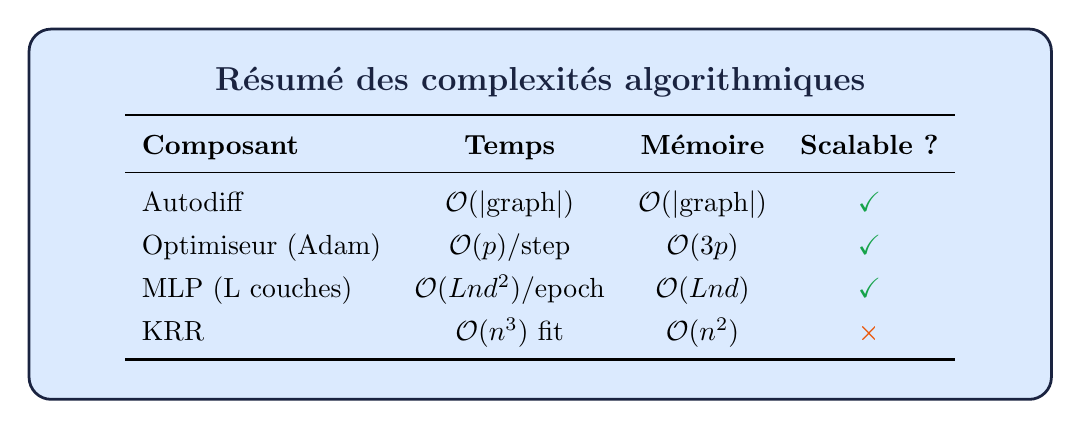
\begin{tikzpicture}
  \node[draw=navyblue, fill=lightblue, rounded corners=8pt,
        inner sep=14pt, line width=1pt] {
    \begin{minipage}{12cm}
      \centering
      {\large\bfseries\color{navyblue} Résumé des complexités algorithmiques}\\[0.5em]
      \renewcommand{\arraystretch}{1.3}
      \begin{tabular}{lccc}
        \toprule
        \textbf{Composant} & \textbf{Temps} & \textbf{Mémoire} & \textbf{Scalable ?}\\
        \midrule
        Autodiff & $\Od(|\text{graph}|)$ & $\Od(|\text{graph}|)$ & \color{defborder}\checkmark \\
        Optimiseur (Adam) & $\Od(p)$/step & $\Od(3p)$ & \color{defborder}\checkmark \\
        MLP (L couches) & $\Od(Lnd^2)$/epoch & $\Od(Lnd)$ & \color{defborder}\checkmark \\
        KRR & $\Od(n^3)$ fit & $\Od(n^2)$ & \color{remarkborder}\texttimes \\
        \bottomrule
      \end{tabular}
    \end{minipage}
  };
\end{tikzpicture}
\end{center}

\vspace{1cm}
\hrule
\vspace{0.4cm}
{\small\color{darkgray}
\textbf{Auteur :} AHNANI Ali \hfill \textbf{Projet :} Mini Framework ML From Scratch\\
\textbf{Outils :} Python 3 $\cdot$ NumPy $\cdot$ Matplotlib \hfill \textbf{Lignes de code :} $\approx$ 1200 (framework) + expériences
}

\end{document}
